\documentclass[a4paper]{article}
\usepackage[a4paper, top=17mm, bottom=17mm, left=17mm, right=17mm]{geometry}
\usepackage[utf8]{inputenc}
\usepackage[T2A,T1]{fontenc}
\usepackage[colorlinks,filecolor=blue,citecolor=green,unicode,pdftex]{hyperref}
\usepackage{cmap}
\usepackage[english,russian]{babel}
\usepackage{amsmath}
\usepackage{amssymb,amsfonts,textcomp}
\usepackage{color}
\usepackage{array}
\usepackage{hhline}
\hypersetup{colorlinks=true, linkcolor=blue, citecolor=blue, filecolor=blue, urlcolor=blue, pdftitle=1, pdfauthor=, pdfsubject=, pdfkeywords=}
% \usepackage[pdftex]{graphicx}
\usepackage{graphicx}
% \usepackage{epigraph}
% Раскомментировать тем, у кого этот пакет есть. Шрифт станет заметно красивее.
%\usepackage{literat}
\usepackage{indentfirst}
\usepackage{wrapfig}

\sloppy
\pagestyle{plain}
%\pagestyle{empty}

\title{Метамоделирование: современный подход к созданию средств визуального проектирования}

\author{А.С. Кузенкова \and Ю.В. Литвинов \and Т.А. Брыксин}
\date{}
\begin{document}

\maketitle
\thispagestyle{empty}

\begin{quote}
\small\noindent
В статье описывается реализация поддержки метапрограммирования в системе QReal. Приводится краткое описание архитектуры системы, процесса создания нового визуального языка метасредствами системы, в том числе приводится описание визуального метаредактора, интеграция метаредактора в среду.
\end{quote}

\section*{Введение}
В настоящее время средства визуального моделирования активно используются для разработки программного обеспечения. Некоторые инструментарии не ориентированы на конкретную предметную область и имеют заранее определенный набор редакторов визуальных языков для создания новых систем. Такие инструментарии называются CASE-пакетами. Их использование само по себе может значительно упростить проектирование сложных систем по сравнению с подходами, основанными на использовании текстовых языков. Но иногда процесс разработки можно ещё более упростить. К примеру, если система проектируется для узко специализированной предметной области, её создание с применением описанного подхода может стать неоправданно трудоёмким процессом. В этом случае уместен другой подход к разработке новых систем --- предметно-орентированное моделирование~\cite{theBook}. Суть его состоит в том, что вместо использования уже имеющихся визуальных языков создается новый язык, специализированный для рассматриваемой предметной области, и система проектируется уже с помощью разработанного языка. Как показывает практика, такой подход является более гибким и удобным~\cite{kieburtz}.

Примерами средств для создания новых предметно-ориентированных языков или DSL (Domain Specific Language) являются Microsoft DSL Tools\footnote{http://msdn.microsoft.com/en-us/library/bb126259.aspx}, Eclipse GMF\footnote{www.eclipse.org/gmf/}, MetaEdit+\footnote{http://www.metacase.com}.

Инструментарий Microsoft DSL Tools используется для создания редакторов визуальных языков, встроенных в среду Visual Studio, и хорошо применим для создания несложных графических редакторов. Создание нового графического редактора состоит в описании его метамодели с возможностью дополнения требуемой функциональности на C\#. Но с помощью него нельзя создать редактор визуального языка, независимый от среды Microsoft Visual Studio.

Технология Eclipse GMF разрабатывается на базе среды разработки Eclipse и также предназначена для создания новых предметно-ориентированных языков, в основном встроенных в эту среду. Но создание метамодели языка в свою очередь требует описания нескольких моделей (доменной, графической модели, моделей инструментов, соответствия и генератора), поэтому процесс создания нового языка является довольно длительным и трудоёмким.

MetaEdit+ является развитым инструментарием для создания DSM-решений, имеет большое число промышленных внедрений. Но цена лицензии на него весьма высока.

Нашей целью была разработка инструментария, сочетающего в себе преимущества существующих и, по возможности, лишенного их недостатков.

\section{QReal}

\begin{wrapfigure}{r}{0.5\textwidth}
  \begin{center}
    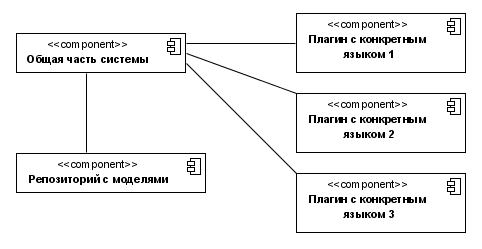
\includegraphics[width=0.5\textwidth]{architecture.jpg}
    \caption{Общая архитектура QReal}
    \label{architecture}
  \end{center}
\end{wrapfigure}

На кафедре системного программирования СПбГУ в течение нескольких лет разрабатывается среда визуального программирования QReal~\cite{qReal}. Разработчики изначально ставили перед собой цель поддержки языка UML 2~\footnote{http://uml.org/}, и на самых ранних этапах разработки поняли, что реализация всех 13 видов диаграмм UML ручным кодированием потребует неоправданно больших усилий. Была разработана следующая схема для упрощения труда программистов: каждая диаграмма языка описывалась на специальном метаязыке (аналогичном языку MOF, на котором описан UML), по XML-файлам с такими описаниями генерировался код на C++, который потом собирался в динамическую библиотеку и подключался к основной части системы как плагин. Такая схема показала себя довольно удобной, и позволила задавать не только диаграммы UML, но и другие существующие визуальные языки с графовой структурой, например, BPEL~\footnote{http://www.ibm.com/developerworks/library/specification/ws-bpel/}, и определять свои собственные визуальные языки. Общая архитектура системы показана на рисунке~\ref{architecture}. Вся информация о синтаксисе языка хранится в плагине, основная часть системы работает в общих для всех языков терминах, модель хранится в репозитории, который тоже ничего не знает о синтаксисе языка, на котором эта модель разработана.

Добавление нового визуального языка в QReal состоит из следующих этапов.
\begin{enumerate}
  \item Автор языка описывает абстрактный и конкретный синтаксис языка (то есть логические сущности в языке, связи между ними, и их внешний вид) в XML-файле. Одному плагину-редактору соответствует один XML-файл, в котором задаются элементы языка, сгруппированные по диаграммам, их логические свойства, взаимоотношения между ними (например, какие элементы могут соединяться какими связями), и описание их графики в формате, похожем на формат SVG. 
  \item Созданное описание добавляется в систему сборки, после чего следующие шаги выполняются при сборке системы автоматически.
  \item По XML-описанию языка генерируется код на C++, реализующий специфику конкретных редакторов и использующий интерфейсы, объявленные в основной части системы.
  \item Сгенерированный код компилируется в динамическую библиотеку, которая помещается в директорию, где основная часть ищет плагины.
  \item При запуске плагин грузится основной частью, сущности нового языка становятся доступны в системе.
\end{enumerate}

Такой способ создания новых графических редакторов в системе имеет ряд принципиальных недостатков. Во-первых, написание XML-файла - это довольно кропотливый процесс, поскольку описание каждого элемента громоздко и не наглядно. Во-вторых, пользователю необходимо обладать определенными знаниями касаемо строения метаметамодели языка и навыками работы с XML.

\section{Метаредактор}
Можно заметить, что XML-описания редакторов можно генерировать по визуальным моделям, тем самым применив технологию предметно-ориентированной разработки саму к себе.

\begin{wrapfigure}{l}{0.25\textwidth}
  \begin{center}
    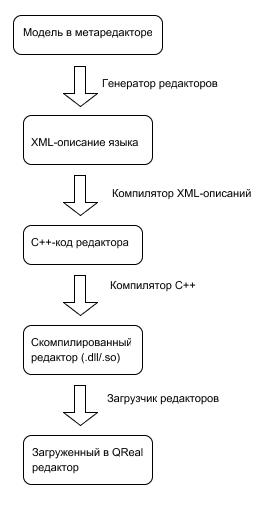
\includegraphics[width=0.25\textwidth]{editorGeneration.jpg}
    \caption{Процесс генерации редактора}
    \label{editorGeneration}
  \end{center}
\end{wrapfigure}

В связи с этим было предпринято расширение инструментов поддержки метамоделирования в QReal. Для этих целей был разработан специальный язык для создания новых визуальных языков (так называемый метаязык), базовыми абстракциями которого являются сущности и отношения. В QReal был создан графический редактор этого визуального языка, где для каждой его абстракции имеется соответствующий элемент. Такой редактор называется метаредактором. Остановимся подробнее на рассмотрении метаязыка и его редактора. 

Плагин может содержать несколько визуальных языков. Плагину в метаязыке соответствует элемент ``Метамодель'', каждому языку --- элемент ``Диаграмма''. Визуальный язык определяется набором своих элементов и взаимосвязей между ними. Основные абстракции делятся на графические и неграфические. К графическим относятся те абстракции, которые обозначают элементы, имеющие графическое представление в редакторе, а к неграфическим, соответственно, не имеющие такового. В метаредакторе графическими являются такие сущности, как ``Элемент'' (Node) и ``Связь'' (Edge), обозначающие, соответственно, элемент визуального языка и связь между элементами. Примером неграфической сущности является ``Перечисляемый тип данных'' (Enum). Она обозначает перечень значений, которые могут использоваться для указания свойств элементов графического редактора. Также с помощью метаредактора можно указывать отношения наследования между элементами на диаграмме и отношения допустимой вложенности одних элементов в другие. Эти отношения на диаграмме указываются стрелками. Помимо этого имеется возможность задавать некоторые дополнительные свойства, поддержка которых осуществлена в QReal (способность “вытягивать” из элементов определенные связи, сортировать вложенные элементы и уметь их скрывать для элементов-контейнеров, и другое). 

Для разработанного языка была создана инструментальная поддержка. После построения метамодели (или нескольких метамоделей) языка пользователь имеет возможность конвертировать его в используемый XML-формат. Была создана инфраструктура, обеспечивающая поддержку сквозного процесса создания графических редакторов. С ее помощью разработчик может спроектировать новый визуальный язык, скомпилировать подключаемый модуль соответствующего графического редактора и подключить его к QReal, не выходя из системы. Также кроме этого реализован разбор существующих XML-файлов и их визуализация с помощью метаредактора, тем самым кроме создания новых визуальных языков пользователь может редактировать уже имеющиеся. Тем самым парсер XML-файлов совместно с генератором в XML-формат позволяет использовать и старый способ задания метамодели языка, то есть данные подходы взаимозаменяемы в зависимости от предпочтений пользователя.

Опишем процесс разработки графического редактора. Он начинается с создания элемента, обозначающего сам редактор, в свойствах которого указывается его название и имя папки, в которой будет сохранен код сгенерированного редактора. Далее создаются диаграммы языков. Внутри каждой диаграммы, используя основные абстракции, задается метамодель языка. У каждого элемента указываются логическое имя, с которым работают генераторы и интерпретаторы моделей, и видимое имя, которое показывается пользователю. Эти имена можно устанавливать взаимонезависимо. Для элементов указываются логические свойства, которые потом можно редактировать в процессе работы с редактором, и они используются для генерации или интерпретации моделей. Задаются отношения наследования и вложенности, указываются дополнительные свойства, которыми обладают элементы. Когда проектирование редактора завершено, пользователь может сразу сгененрировать редактор. Если имеются некоторые ошибки в проектировании (к примеру, не указаны необходимые свойства абстракций), то сообщения о них появятся в специальном окне, и имеется возможность их исправить. Если же всё сделано правильно, пользователю предлагается сразу подключить редактор к среде.  

Процесс сборки нового языка в QReal схематически изображён на рисунке~\ref{editorGeneration}

\section{Заключение}
Описанный в статье метаредактор реализован и используется в системе QReal для создания новых визуальных языков. Один из примеров языка, разработанного с помощью метаредактора --- язык программирования роботов Lego Mindstorms NXT\footnote{http://mindstorms.lego.com}. Этот визуальный язык позволяет задавать логику поведения робота в виде последовательности управляющих блоков, таких как ``Включить мотор на таком-то порту с такой-то мощностью'', и исполнить программу на роботе, интерпретируя диаграмму и посылая команды роботу через Bluetooth. Визуальный язык прост и понятен, что даёт возможность его использовать даже ученикам начальной школы. Пример диаграммы на этом языке изображён на рисунке~\ref{robotsDiagram}. Метамодель этого языка несложная, добавить новый элемент в язык чрезвычайно просто --- перетащить элемент с палитры, задать его свойства, нарисовать в редакторе его внешний вид, сгенерировать редактор и тут же начать новый элемент использовать.

\begin{figure} [ht]
  \begin{center}
    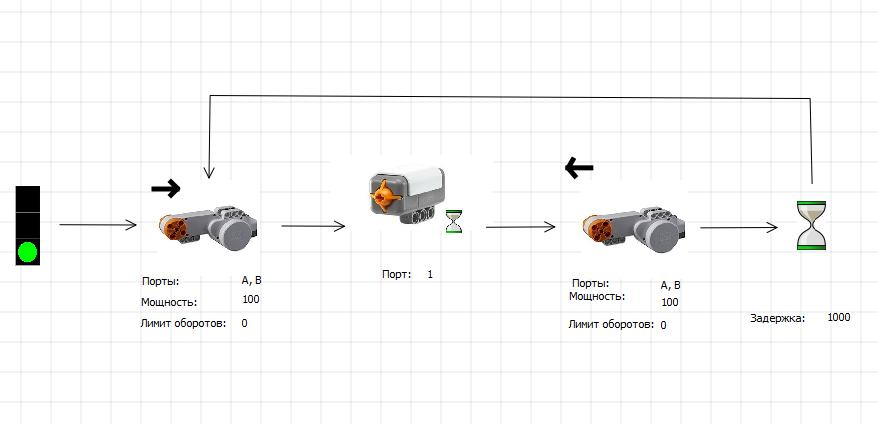
\includegraphics[width=0.8\textwidth]{robotsDiagram.jpg}
    \caption{Диаграмма поведения робота}
    \label{robotsDiagram}
  \end{center}
\end{figure}

%\begin{figure} [ht]
%  \begin{center}
%    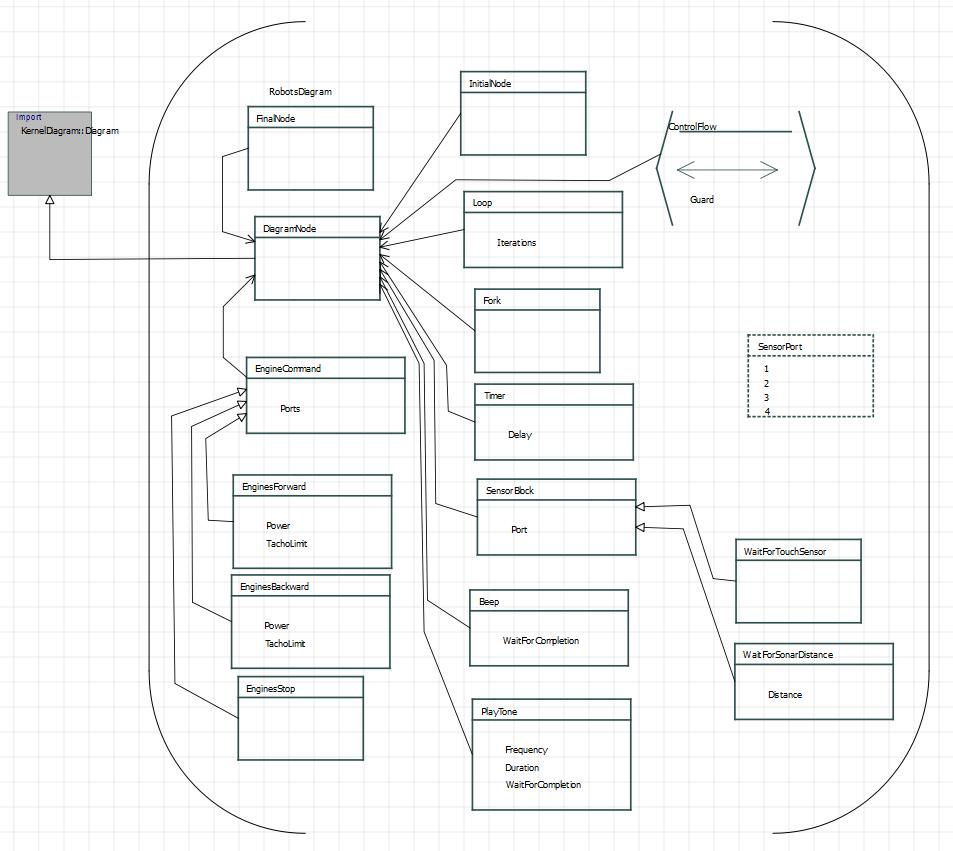
\includegraphics[width=0.6\textwidth]{robotsMetamodel.jpg}
%    \caption{Метамодель редактора диаграмм роботов}
%    \label{robotsMetamodel}
%  \end{center}
%\end{figure}

\begin{thebibliography}{9001}
  \bibitem{qReal} А.Н. Терехов, Т.А. Брыксин, Ю.В. Литвинов и др., Архитектура среды визуального моделирования QReal. // Системное программирование. Вып. 4. СПб.: Изд-во СПбГУ. 2009, С. 171-196
	\bibitem{kieburtz} Kieburtz, R., et al. A software engineering experiment in software component generation, Proceedings of 18th International Conference on Software Engineering, Berlin, IEEE Computer Society Press, March, 1996
  \bibitem{theBook} Kelly, S., Tolvanen, J. Domain-Specific Modeling: Enabling Full Code Generation // Wiley-IEEE Computer Society Press. 2008. 448 pp.
\end{thebibliography}

\end{document}